\documentclass[11pt]{article}
\usepackage{amsmath,amsthm,amsfonts,amssymb}
\usepackage[margin=1in]{geometry}
\usepackage{fancyhdr}
\usepackage{hyperref}
\usepackage{xcolor}
\usepackage{tcolorbox}

\usepackage{tcolorbox}
\usepackage{enumerate}
\usepackage{tikz}


\usepackage{algorithmic}

\usetikzlibrary{arrows.meta}

    \setlength{\headheight}{26pt}
    \pagestyle{fancy}
    \fancyhead[C]{\textbf{Basic Algorithms (Section 5)}\\Spring 2025}
    \fancyhead[R]{HW10 (Due 4/24 23:59)\\ Instructor: Jiaxin Guan}
    \fancyfoot[C]{}
    \fancyfoot[R]{\thepage}
    \renewcommand{\headrulewidth}{0.4pt}
    \renewcommand{\footrulewidth}{0.4pt}  
    

\begin{document}


    %%%% EDIT THIS PART 
    %Put your name and Net ID here
    \fancyhead[L]{Name:  \\ Net ID: }
    %Write your collaborators' names here
    \fancyfoot[L]{Discussion Partners:}
    %%%%%

    %Problem 1
    \begin{tcolorbox}[title={Problem 1 (Topological Sort, 25 pts)}] \setlength\parindent{1em}
         How many valid topological sorts does the directed graph below have? List all the valid topological sorts in the following table. One of them has been listed as an example, where node A is output first and D is output last.

        \centering

        \vspace{2em}
        \begin{tabular}{ccccccc}
            \hline
             1. & A & B & C & F & E & D \\
             2. &  &  &  &  &  & \\
             &  &  &  &  &  & \\
             &  &  &  &  &  & \\
             &  &  &  &  &  & \\
             &  &  &  &  &  & \\
             &  &  &  &  &  & \\
             &  &  &  &  &  & \\
             &  &  &  &  &  & \\
            \hline
        \end{tabular}

        \vspace{2em}
        \begin{tikzpicture}[>={Latex[width=3mm,length=3mm]},
                node distance=1.5cm,
                scale=2,
                thick,main/.style = {draw, circle}]
            % Nodes
            \node[main,scale=1.8] (A) {A};
            \node[main,scale=1.8] (B) [above right of=A] {B};
            \node[main,scale=1.8] (C) [right of=B] {C};
            \node[main,scale=1.8] (D) [below right of=C] {D};
            \node[main,scale=1.8] (E) [below left of=D] {E};
            \node[main,scale=1.8] (F) [below right of=A] {F};

            %Edges
            \draw[->] (A) -- (B);
            \draw[->] (A) -- (F);
            \draw[->] (B) -- (C);
            \draw[->] (B) -- (F);
            \draw[->] (E) -- (D);
            \draw[->] (B) -- (D);
            \draw[->] (C) -- (F);
            \draw[->] (C) -- (D);
            \draw[->] (C) -- (E);
        \end{tikzpicture}
        \vspace{0.5em}
    \end{tcolorbox}

    %Write your solution here!
    
    \newpage
    %Problem 2
    \begin{tcolorbox}[title={Problem 2 (Reachability, 35 pts)}] \setlength\parindent{1em} 
        Suppose you are given a directed graph $G=(V,E)$ where each vertex, $u\in V$, is labeled with a unique value $L(u)$ from the set $\{1,\ldots,|V|\}$. For each vertex $u$, let $R(u)$ denote the set of vertices \emph{reachable} from $u$ in $G$. Define $\max(u)$ to be the \emph{vertex} $v^*_u$ in $R(u)$ with the maximum label, i.e.~$L(v^*_u) \ge L(v)$ for all $v\in R(u)$.
        
        Give an $O(|V|+|E|)$ time algorithm to compute $\max(u)$ for all vertices in $u\in V$. Briefly justify correctness and runtime of your algorithm.
    \end{tcolorbox}
    
    %Write your solution here!

    \newpage
    %Problem 3
    \begin{tcolorbox}[title={Problem 3  (Helping Botanical Garden, 40 pts)}]

    Suppose the New York Botanical Gardens are trying to drum up interest for their tree and shrub collections by offering tours through the arboretum, and you are tasked with reviewing their proposed routes. There are a set $V$ of trees they want some tour to stop at, and a set $E$ of routes from tree to tree their proposed tours would make. In order to make sure all the trees are visited, they want the following property:

    \begin{center}
        \textit{For all pairs $u, v \in V$ such that $u \neq v$, we must have a path from $u$ to $v$ \textbf{or} a path from $v$ to $u$ (or both).}
    \end{center}

    \textbf{Notice how this property is different from strongly connectedness.} They provide you and your classmates with many proposed plans and a strict deadline for your feedback, and so you want to develop an efficient algorithm to automate this task.

    \begin{enumerate}[(a)]
        \item Suppose $G = (V, E)$ is a directed acyclic graph (DAG). Your classmates propose two possible algorithms to determine whether or not the given graph $G$ satisfies the desired property. For each of the proposed algorithms below, \textbf{analyze its runtime and whether it is correct. If it is correct, give a justification. If it is incorrect, provide a counterexample.}
        \begin{enumerate}[(i)]
            \item Student A proposes the following algorithm: First, find a source vertex $s$ in the graph that has no incoming edges. If there are multiple sources, pick an arbitrary one. Then, run a \textbf{DFS-Visit} (notice this is only the recursive portion of DFS, not the entire DFS) on $G$ starting from $s$. $G$ satisfies the property if and only if the DFS-Visit visits all the vertices in the graph.
            \item Student B proposes the following algorithm: First, run DFS on the graph to obtain a topological sort of the vertices. Let the topological sort be $v_1, v_2,\dots, v_n$. Then, we check for the following edges $(v_1, v_2), (v_2, v_3), (v_3, v_4), \dots, (v_{n-1}, v_n)$. If all of these edges exist, then we say $G$ satisfies the property. If any of the edges are missing, we say $G$ does not satisfy the property.
        \end{enumerate}
        \item Now you want to generalize the algorithm to work for \textbf{any} directed graph. Design a $O(|V|+|E|)$ time algorithm to determine whether or not the given graph $G$ satisfies the desired property. You may use the algorithms from part (a) as a subroutine.  Make sure to justify the correctness and runtime of your proposed algorithm.
    \end{enumerate}
    \end{tcolorbox}
    
    %Write your solution here!
    
\end{document}